The alignment procedure uses track-based algorithm that updates the locations of detector elements in order to minimize the set of track-hit \emph{residuals}.
These residuals are defined as the distance between the fitted track position in a given detector element to the position of the hit recorded by the same element.
Tracks in ATLAS are parameterized as five-dimensional vectors~\cite{2006.atlas-tracking-model}:%follow helical trajectories and are parameterized as five-dimensional vectors~\cite{2006.atlas-tracking-model}:
\begin{equation}
  \vec{\tau} = (d_0,z_0,\phi_0,\theta,q/p)
\end{equation}
where $d_0$ and $z_0$ are the transverse and longitudinal impact parameters with respect to the origin, respectively, $\phi_0$ is the azimuthal angle of the track at the point of closest approach to the origin, $\theta$ is the polar angle, and $q/p$ is the charge of the track divided by its momentum.
The residual for the $i^{\textrm{th}}$ hit of a given track can then be written in terms of the track parameters $\vec{\tau}$ and a set of alignment parameters $\vec{a}$ that describe the hit location~\cite{2005.global-chi2-alignment}:
\begin{equation}
  r_i(\vec{\tau},\vec{a}) = (\vec{m}_i - \vec{e}_i (\vec{\tau},\vec{a}))\cdot\hat{k}
\end{equation}
where $\vec{e}_i$ is the intersection point of the extrapolated track with the sensor, $\vec{m}_i$ is the position of the associated hit within the sensor, and $\hat{k}$ is the unit vector defining the direction of the measurement within the sensor.
$\vec{r}$ is then the vector of residuals for the given track.

% the alignment constants are those that minimize the track-hit residuals
A $\chi^2$ function can be built from the residuals of all collected tracks:
\begin{equation}
  \chi^2 = \sum\limits_{\textrm{tracks}}\vec{r}^{T}V^{-1}\vec{r}
  \label{eq:alignment_chi2}
\end{equation}
where $V$ is the covariance matrix of the hit measurements.
The $\chi^2$ function is then minimized with respect to the alignment parameters $\vec{a}$, which contain all degrees of freedom being aligned.
The minimzation condition with respect to $\vec{a}$ is:
\begin{equation}
  \frac{d\chi^2}{d\vec{a}} = 0 ~~ \rightarrow ~~ 2\sum\limits_{\textrm{tracks}}\bigg(\deriv{\vec{r}}{\vec{a}}\bigg)^{T}V^{-1}\vec{r} = 0
  \label{eq:alignment_chi2_min_condition}
\end{equation}
This equation can be difficult to solve exactly, so the residual is rewritten as a first order Taylor expansion:
\begin{equation}
  %\vec{r} = \vec{r}_0+\frac{\partial\vec{r}}{\partial\vec{\tau}}\delta\vec{\tau}+\frac{\partial\vec{r}}{\partial\vec{a}}\delta\vec{a}
  \vec{r} = \vec{r}_0+\deriv{\vec{r}}{\vec{a}}\delta\vec{a}
  \label{eq:alignment_residual_taylor}
\end{equation}
where $\vec{r}_0$ is dependent on an initial set of track and alignment parameters $\vec{\tau}_0$ and $\vec{a}_0$, respectively; the track parameter dependence has also been folded into the total derivative $\deriv{\vec{r}}{\vec{a}}$.
Equation~\ref{eq:alignment_residual_taylor} can then be inserted into the minimization condition from Equation~\ref{eq:alignment_chi2_min_condition} to give:
\begin{equation}
  \Bigg[ \sum\limits_{\textrm{tracks}}\bigg(\deriv{\vec{r}}{\vec{a}}\bigg)^{T}V^{-1}\bigg(\deriv{\vec{r}}{\vec{a}}\bigg) \Bigg]\delta\vec{a} + \sum\limits_{\textrm{tracks}}\bigg(\deriv{\vec{r}}{\vec{a}}\bigg)^{T}V^{-1}\vec{r}_0 = 0
  \label{eq:alignment_chi2_min_taylor}
\end{equation}
From this equation, the alignment matrix $\mathcal{M}_a$ and alignment vector $\vec{\nu}_a$ can be defined:
\begin{equation}
  \mathcal{M}_a = \sum\limits_{\textrm{tracks}}\bigg(\deriv{\vec{r}}{\vec{a}}\bigg)^{T}V^{-1}\bigg(\deriv{\vec{r}}{\vec{a}}\bigg)
  \label{eq:alignment_matrix}
\end{equation}
\begin{equation}
  \vec{\nu}_a = \sum\limits_{\textrm{tracks}}\bigg(\deriv{\vec{r}}{\vec{a}}\bigg)^{T}V^{-1}\vec{r}_0
  \label{eq:alignment_vector}
\end{equation}
Finally, the alignment corrections $\delta\vec{a}$ can be solved for by inverting the alignment matrix:
\begin{equation}
  \delta\vec{a} = -\mathcal{M}_a^{-1}\vec{\nu}_a
  \label{eq:alignment_corrections}
\end{equation}
%The \emph{alignment constants} are the values of $\vec{a}$ that minimize the track-hit residuals.
which is a linear system of equations with a number of equations equal to the number of alignment degrees of freedom~\cite{2011.alignment-7tev}.

Inverting the matrix and solving this system of equations is referred to as \emph{Global} $\chi^2$ alignment~\cite{2005.global-chi2-alignment}.
This can be useful, as $\mathcal{M}_a$ contains all the correlations between the alignable structures.
However, inverting the matrix becomes difficult when the number of degrees of freedom becomes large, and
%There are several different \emph{levels} of alignment of increasing granularity, which will be outlined in detail in Section~\ref{align:levels}.
as the number of alignable structures increases, so too does the size of the matrix $\mathcal{M}_a$.
Eventually inverting the matrix becomes too computationally intensive to be practical.

This problem is solved by the \emph{Local} $\chi^2$ algorithm~\cite{2005.local-chi2-thesis}.
In this case, the alignment matrix is constructed to be block-diagonal, allowing for it to be inverted even for large numbers of degrees of freedom.
This is achieved by replacing the full derivative in Equation~\ref{eq:alignment_chi2_min_taylor} with the partial derivative $\frac{\partial\vec{r}}{\partial\vec{a}}$.
The new alignment matrix $\mathcal{M}'_{a}$ and alignment vector $\vec{\nu}'_a$ become:
\begin{equation}
  \mathcal{M}_a = \sum\limits_{\textrm{tracks}}\bigg(\pderiv{\vec{r}}{\vec{a}}\bigg)^{T}V^{-1}\bigg(\pderiv{\vec{r}}{\vec{a}}\bigg)
  \label{eq:alignment_matrix_local}
\end{equation}
\begin{equation}
  \vec{\nu}_a = \sum\limits_{\textrm{tracks}}\bigg(\pderiv{\vec{r}}{\vec{a}}\bigg)^{T}V^{-1}\vec{r}_0
  \label{eq:alignment_vector_local}
\end{equation}
Inverting $\mathcal{M}'_{a}$ is considerably faster and less intensive even for large numbers of degrees of freedom; however, the correlations between the alignable structures is lost.

Due to the Taylor expansion used in Equation~\ref{eq:alignment_chi2_min_taylor}, several iterations of the alignment algorithm may be necessary to converge on a final set of alignment constants.
The Local $\chi^2$ alignment typically requires more iterations due to the loss of the correlation information~\cite{2007.alignment-strategy}.
In practice, the ATLAS reconstruction is run over a set of events, and the resulting tracks are fed to the alignment algorithm.
The residuals are calculated, the alignment matrix is built and inverted, and a new set of alignment constants is obtained.
The convergence of the alignment can be checked by:
\begin{enumerate}
\item Measure the $\Delta\chi^2$ with the previous iteration. If it is near zero, then the $\chi^2$ is approaching its minimum.
\item Looking at the residual distributions for different alignable structures. A well aligned detector will have a mean residual of zero with a width approximating the intrinsic resolution of the detector.
\end{enumerate}
If the above checks are satisfied, the process is finished and the final alignment constants are read out; if not, another iteration is performed.
A visual representation of the alignment chain is shown in Figure~\ref{fig:alignment_chain}.

\begin{figure}[htbp]
  \centering
  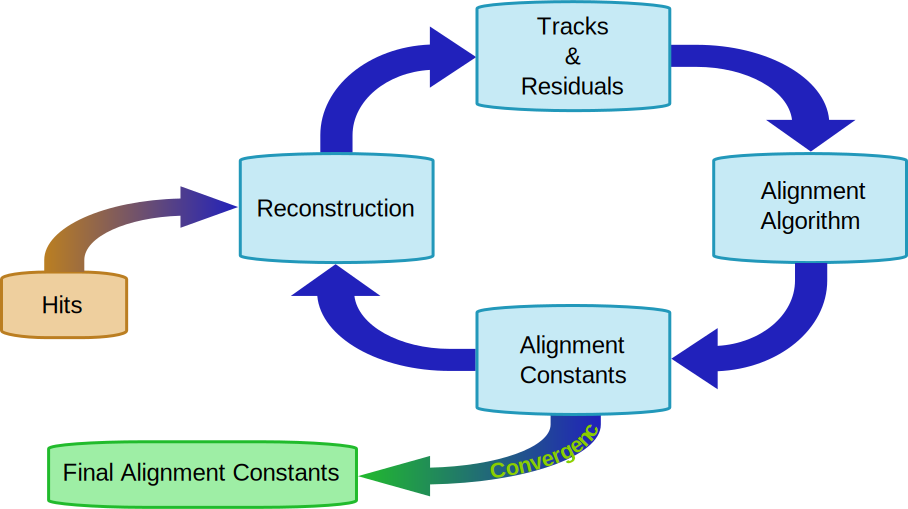
\includegraphics[width=.8\textwidth]{figs/alignment/alignment-chain}
  \caption{Graphical representation of the ID alignment chain.}
  \label{fig:alignment_chain}
\end{figure}

Since a $\chi^2$ minimization is used to align the detector, if there is a systematic misalignments in the detector that does not adversely affect the $\chi^2$, the algorithm will be insensitive to it.
These misalignments are referred to as \emph{weak modes}, and special care is taken to remove them~\cite{2014.alignment-performance-8tev}.
One potential impact of weak modes is a bias in the track momentum of reconstructed particles.
This particular effect is the subject of Section~\ref{align:bias}.

In practice, the detector is aligned both in ``real-time'' as data is collected, and during dedicated offline alignment campaigns.
The real-time alignment is run in ATLAS's so-called \emph{calibration loop}, which comprises the first stage in the preparation of data for physics analysis.
The calibration loop requires the alignment as well as various other detector calibrations to be available within 48 hours for initial data processing.
A fast, coarse-grained alignment\footnote{The calibration loop runs up to a Level 2 alignment in the silicon detectors, which involves treating each layer of sensors as a single object, defined in greater detail in Table~\ref{tab:align_levels}.} is run on a subset of the available data containing full tracking information, and the results are propagated to the reconstruction of that particular run~\cite{2015.alignment-run-2-proceedings}.
Due to the time constraints of the calibration loop, a full sensor-by-sensor alignment is not possible.

The more thorough and finely tuned alignments are reserved for the dedicated alignment campaigns.
These generally occur early in data taking campaigns, typically once a sufficient amount of data is collected after a detector shutdown, in order to obtain a good baseline alignment for use in the remainder of the data collection period.
Once data taking is complete, another campaign determines an improved set of alignment constants (divided into several ``blocks'' to account for time-dependent misalignments), and the full data is reprocessed using the newly derived detector geometry.
The initial offline alignment of the ATLAS detector at the beginning of Run 2 in 2015 is the subject of Section~\ref{align:2015}.

\subsection{Alignment levels}\label{align:levels}
The alignment of the detector is performed at several levels of increasing granularity.
This adds flexibility in being able to align only as finely as needed, and it also allows for global, detector-level misalignments to be corrected first before dealing with finer adjustments.
\begin{itemize}%[{Level }1:]
\item Level 1 (L1) alignment involves moving entire subdetector components as a single unit, such as the entire Pixel detector, or the SCT barrel.  These often have the largest misalignments, but they are easily corrected and do not require large volumes of data to do so.
\item Level 2 (L2) alignment treats individual layers in the silicon detectors (modules in the TRT) and end cap disks as individual alignable objects.
\item Level 2.7 (L27) alignment was introduced with the addition of the IBL to the ID in Run 2.  It involves the stave-by-stave alignment of the IBL and Pixel barrel\footnote{For the purposes of this Chapter, the term ``Pixel'' will refer to the original three layers of the Pixel detector, and the IBL will be referenced separately.}.
\item Level 3 (L3) alignment treats each sensor in the silicon detectors and each straw in the TRT as an individual alignable object.  It is the finest grained alignment available but also the most computationally intensive due to the large number of degrees of freedom.  The large number of individual detector sensors being aligned also requires the largest amount of statstics.
\end{itemize}
The different alignment levels are listed in more detail in Table~\ref{tab:align_levels}, including the number of alignable structures and associated degrees of freedom for each detector component.

The implementation of the alignment algorithm in the software is flexible enough to allow each subsystem to be aligned individually at a specified level.
Each alignable structure has six degrees of freedom: 3 translations ($T_x$, $T_y$, $T_z$) and 3 rotations ($R_x$, $R_y$, $R_z$)\footnote{The TRT is an exception, as the subdetector does not have any resolution along the length of the straw.  Therefore, for the barrel, $T_z$ is omitted.  Similarly for the straws themselves, only two parameters are defined: translation with respect to the radial direction ($T_\phi$) and rotation with respect to the radial axis ($R_r$ for the barrel and $R_z$ for the end-caps)~\cite{2012.johnda-thesis}.}; however individual degrees of freedom may be turned on and off as required.
In a typical alignment job, L1 and L2 contain few enough degrees of freedom that the Global $\chi^2$ algorithm can be used, but L3 alignments (which can contain over 36,000 degrees of freedom in the silicon detectors alone) require the Local $\chi^2$ algorithm.

\begin{table}[htbp]
  \centering
    \resizebox{\textwidth}{!}{
    \begin{tabular}{c|lr|rr}
    Level & Description of alignable structure & & Structures & DoF \\
    \hline\hline
    \multirow{5}{*}{1} & IBL detector                                                  & & 1 & 6 \\
      & Whole Pixel detector & & 1 & 6 \\
      & SCT barrel and 2 end-caps & & 3 & 18 \\
      & TRT barrel and 2 end-caps ($T_z$ fixed) & & 3 & 17 \\ \cline{3-5}
      &  & Total: & 8 & 47 \\
    \hline
    \multirow{8}{*}{2}  & IBL detector  & & 1 &  6 \\
       & Pixel barrel layers & & 3 & 18 \\
       & Pixel end-cap disks & & $2\times 3$ & 36 \\
       & SCT barrel layers & & 4 & 24 \\
       & SCT end-cap disks & & $2\times 9$ & 108 \\ 
       & TRT barrel 32 modules ($T_z$ fixed) & & $ 3 \times 32$ & 480 \\ 
       & TRT end-cap wheels & & $ 2 \times 40$ & 480 \\ \cline{3-5}
       &  & Total: & 208 & 792 \\
    \hline
    \multirow{4}{*}{2.7} & IBL staves  & & 14 & 84 \\
        & Pixel barrel staves & & 22+38+52 & 672 \\
        & Pixel end-cap disks  & & $2\times 3$ & 18 \\ \cline{3-5}
        & & Total: & 132 & 1,878 \\
    \hline
    \multirow{7}{*}{3}  & IBL modules    & & 280 &  1,680 \\            
       & Pixel modules  & & 1,744 & 10,464 \\
       & SCT modules   & & 4,088 & 24,528 \\ 
       & TRT barrel wires ($T_\phi, R_r$ only)  & & 105,088 & 210,176\\ 
       & TRT end-cap wires ($T_\phi, R_Z$ only)  & & 245,760 & 491,520\\ 
    \cline{3-5}
        & & Total silicon sensors: & 6,112 & 36,672 \\
        & & Total TRT wires: & 350,848 & 701,696 \\
    \hline
  \end{tabular} 
  }
  \caption{The four alignment levels for each of the detector subsystems. The total number of alignable structures and degrees of freedom (DoF) to be aligned are given for each level.}
  \label{tab:align_levels}
\end{table}

\subsection{Alignment coordinate systems}\label{align:coords}
The global coordinate system ($x$, $y$, $z$) used by the ID alignment matches that of the ATLAS detector in general, as detailed in Section~\ref{sec:atlas} \TODO{update with actual location of figure when it's in...}.
The positions and orientations of individual detector modules of the ID are defined by a right-handed local coordinate system ($x'$, $y'$, $z'$) where the origin is defined as the geometrical center of the module.
The $x'$-axis for each silicon module is defined to point along the most sensitive direction of the module, the $y'$-axis is oriented along the long side of the module, and the $z'$-axis is orthogonal to the ($x'$, $y'$) plane.
For the TRT straws, the $x'$-axis is perpendicular to both the wire and the radial direction, defined from the origin of the global frame to the straw center, the $y'$-axis points along the straw, and once again the $z'$-axis is orthogonal to the ($x'$, $y'$) plane.
A depiction of the global and local coordinate systems for the ID is shown in Figure~\ref{fig:align_coords}.

When considering the alignment degrees of freedom listed earlier in Section~\ref{align:levels}, grouped collections of modules, layers, or entire subdetectors use the global coordinate system; individual modules use their respective local coordinate systems.
The translations $T_i$ are with respect to the origin of the given reference frame, and the rotations $R_i$ are taken about the Cartesian axes.

\begin{figure}
  \centering
  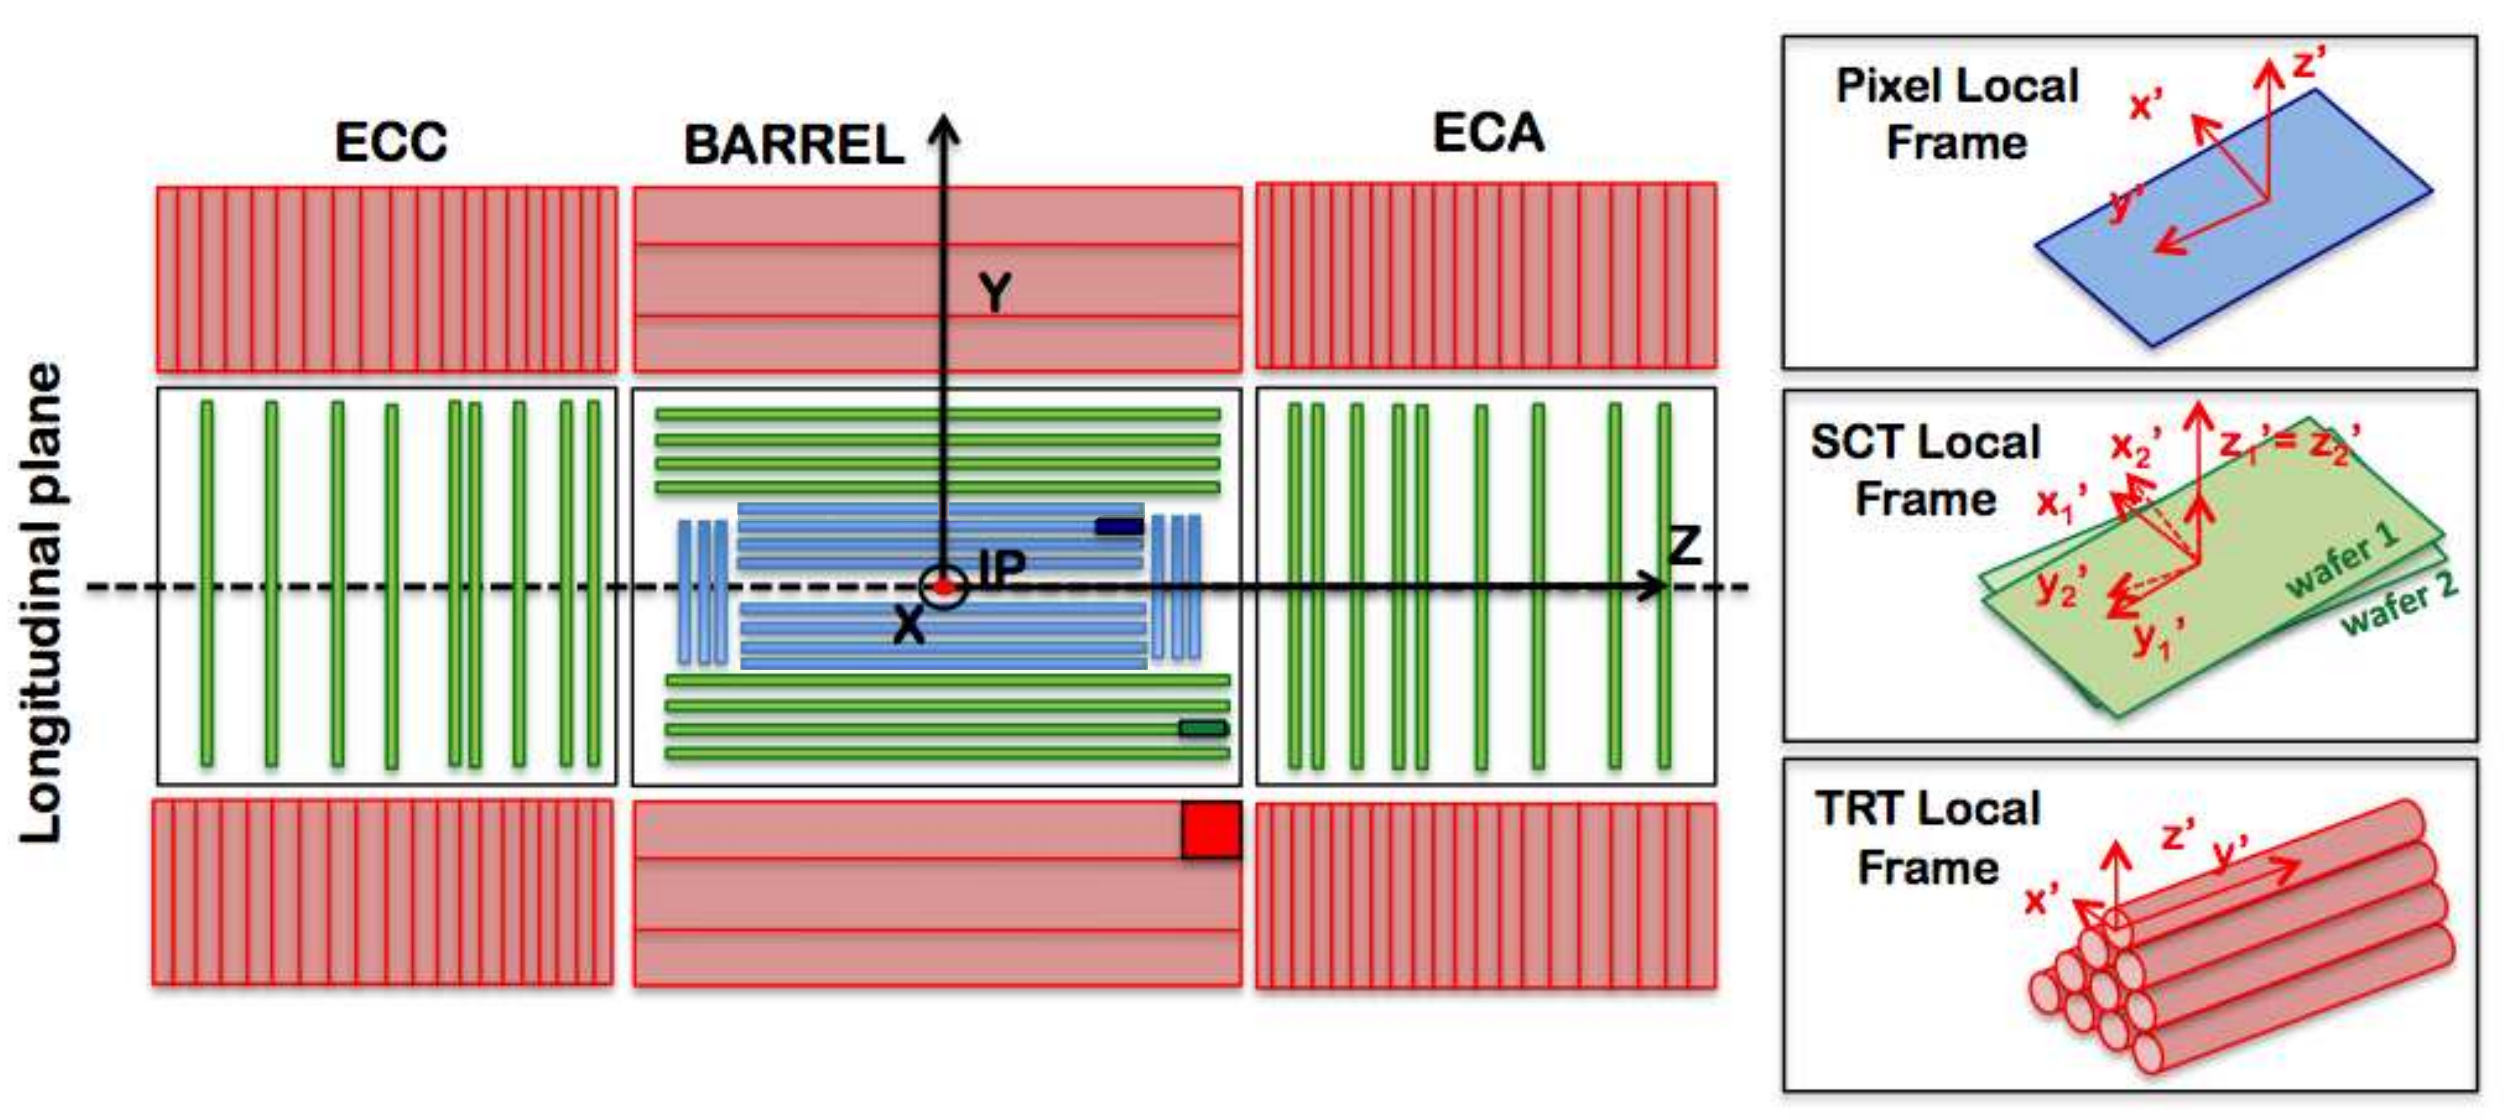
\includegraphics[width=.8\textwidth]{figs/alignment/ReferenceFrame}
  \caption{A schematic representation of the Inner Detector in the longitudinal plane with the global coordinate system overlaid on top.  The Pixel detector and IBL are shown in blue, the SCT in green, and the TRT in red.  The local coordinates for each subdetector module are inset on the right.  Image taken from~\cite{2015.alignment-2015-cosmic}.}
  \label{fig:align_coords}
\end{figure}
